\chapter{Approach}\label{chap:approach}
The approach starts with the problem definition and continues with what you have done. Try to give an intuition first and describe everything with words and then be more formal like `Let $g$ be ...'.

Strive to make the following items crystal clear to your readers.
\begin{itemize}
\item What is the problem you are treating?
\item What are the research questions you want to answer in this work?
\item What are your own contributions and what is work of others? If
  you are working in a team, it is important to demarcate against the
  contributions of others in your team.
\end{itemize}

Describe each major technical problem and how it was solved.

\section{Problem Definition}
\todo{JavaScript popularity has increased dramatically over the last years. TypeScript has evolved naturally as the professional way of developing code in JavaScript, providing the robustness that ervery compiled language has. Generating the declaration files manually is very time consuming and error prone.}

\todo{NodeJS, frameworks like React, Angular, Vue. The migation to Single Page Apps and Serverless, etc.}

\todo{Info from Stackoverflow and Github}

\todo{Mention DefinitelyTyped repository. Explicar claramente que el objetivo de esta tesis es generar }

\todo{El objetivo es solucionar el problema de definitely typed!!! Por eso se usa como objetivo que el input sea un node module}

\section{TypeScript Declaration Files Generation Method}
\todo{Explain overview process for generating declaration file.  Explain that the focus of this thesis was to focus on the runtime information and use the symbolic executor as a 'refinement' of the test cases. Use 'public' document of the Master project}

This Thesis introduces a \textit{TypeScript Declaration Files Generation Method}, which generates a valid TypeScript Declaration File for a specific NPM package, as explained in \figref{fig:tsd_generation_method_block_diagram}.

\begin{figure}[h]
\begin{centering}
    {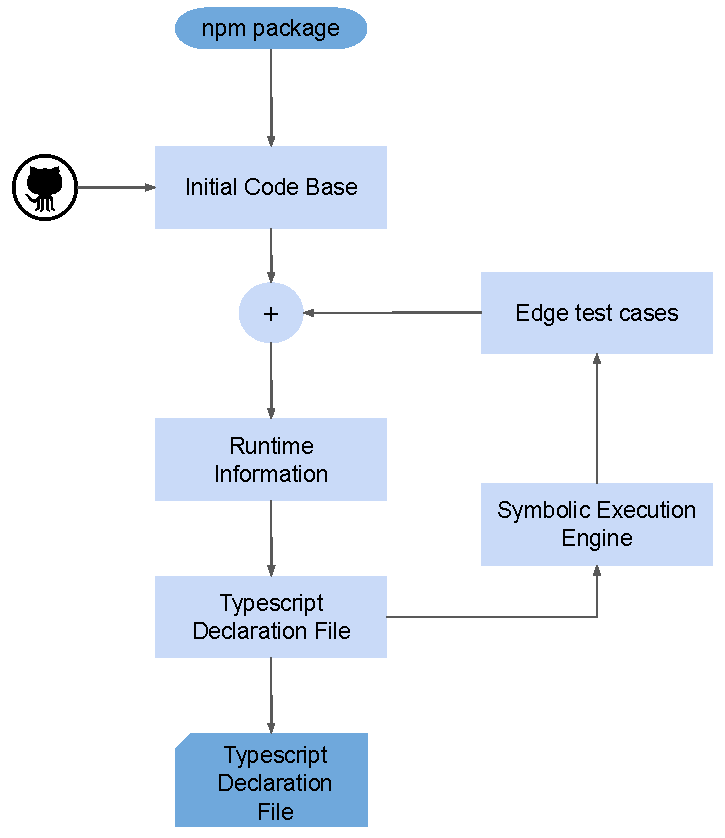
\includegraphics[width=0.9\textwidth]{figures/approach/typescript-declaration-files-generation-method/typescript_declaration_files_generation_method_block_diagram.pdf}}
    \caption[TypeScript Declaration Files Generation Method]{\textbf{TypeScript Declaration Files Generation Method} - Initial code base is retrieved from the npm package's repository. A valid TypeScript Declaration File is generated using run-time information. A Symbolic Execution Engine creates test cases based on the generated Declaration File and via a feedback loop enriches the code base until the stopping criteria is reached. The final TypeScript Declaration File gets returned.}
    \label{fig:tsd_generation_method_block_diagram}
\end{centering}
\end{figure}


Following the goal of easing and automating the generation of TypeScript Declaration Files for existings JS Libraries, the method receives the name of the JS Library published to the NPM Registry as an input argument and returns the corresponding TypeScript declaration file.

The method consists of a continuous refinement process. It generates a TypeScript Declaration File based on data flow and type information gathered at run-time from a code base that executes the JS Library. A Symbolic Execution Engine expands the code base in every iteration by generating new test cases that explore different execution paths.

The file generated after each iteration is a valid and fully functional declaration file, suitable for usage in development environments. It contains no errors, matches the structure of the corresponding JS Library and could be uploaded to the DefinitelyTyped Repository. It is therefore intended to be integrated within the build process of the JS Library.

The feedback loop is not included in the implementation. Exploring new execution paths by creating new test cases will refine the declaration files, i.e. new types will be assigned to different variables, new interfaces will be detected, existing interfaces will be defined more accurately by detecting new properties, etc. From an incremental point of view, actually generating the declaration files from run-time information has to be developed first. A declaration file must exist first so that it can be refined refined afterwards. 



\todo{Decir que para la tesis se decidio no inlcuir el feedback loop. Solo se hizo la parte de runtime, etc.}

\subsection{Implementation}
As explained before, the DefinitelyTyped Repository is the official repository for finding declaration files for npm packages. Therefore, the \textit{TypeScript Declaration Files Generation Method} is intended to be used on existing, published npm packages. The generated output TypeScript declaration file is a valid file which can be used for development and uploaded to the DefinitelyTyped Repository.

The method uses Jalangi as instrumentation framework to gather data flow information and type information at runtime. A second independent block uses the gathered information to generate a TypeScript Declaration File. The signatures obtained from the generated declaration file are used to generate pre and post conditions on a Symbolic Execution Engine in order to build different test cases that explore new execution paths. The code from the test cases is then added to the existing code base. The declaration file is generated again using an expanded code base.

A feedback loop refines iteratively the outcome by combining run-time information gathering and symbolic analysis: It performs Run-Time Analysis to generate a declaration file using run-time information and a Symbolic Execution Engine to refine and expand the code base being used to gather run-time information.

Running the TypeScript Declaration File Generation Tool with the same run-time information as input will always produce the same result. If new execution paths are covered by the test cases, new run-time information will be gathered and the declaration file will change accordingly. In order to obtain a sound analysis, this feedback loop would be iterated until there are no differences among the generated declaration files. However, by trading soundness for scalability, the overall procedure can be stopped either using a loop bound, a time bound or an heuristics mechanism. Exploring and investigating the proper stopping criteria is beyond the scope of this work.  

Finally, the generated declaration files are fully functional and valid files. They can be used in a TypeScript project without further modifications

\todo{Decir que es un framework. Decir que es tipo una pipeline donde todo se conecta con lo otro. Explicar que por mas que reciba un string como input}

\section{Initial code base}

\section{Run-time Information Gathering} \label{run-time-information-gathering}
\subsection{Instrumentation}
\subsubsection{Interactions}
\todo{inputValue}
\todo{getField}
\todo{putField}
\todo{methodCall}
\todo{usedAsArgument}
\todo{convertedTo}

\subsubsection{Wrapper Objects}
\todo{Proxy Objects}
\todo{Primitives}
\todo{Null}
\todo{Undefined}
\subsection{Output Format}
\todo{Explicar que es un JSON con todas las interactions. Explicar estructura de cómo se forma el JSON}
\subsection{Blacklisted Modules}
\begin{figure}[tp]
	\centering
	\begin{lrbox}{\mintedbox}
		\begin{minipage}{0.45\textwidth}
			\jscode{code/blacklisted-modules/foo.js}
		\end{minipage}
	\end{lrbox}
	\subfloat[foo/index.js]{\usebox{\mintedbox}}
	\hfill
	\begin{lrbox}{\mintedbox}
		\begin{minipage}{0.45\textwidth}
			\jscode{code/blacklisted-modules/A.js}
		\end{minipage}
	\end{lrbox}
	\subfloat[A/index.js]{\usebox{\mintedbox}}

	\begin{lrbox}{\mintedbox}
		\begin{minipage}{0.48\textwidth}
			\jscode{code/blacklisted-modules/D.js}
		\end{minipage}
	\end{lrbox}
	\subfloat[D/index.js]{\usebox{\mintedbox}}
	\hfill
	\begin{lrbox}{\mintedbox}
		\begin{minipage}{0.45\textwidth}
			\jsoncode{code/blacklisted-modules/blacklist.json}
		\end{minipage}
	\end{lrbox}
	\subfloat[blacklist.json]{\usebox{\mintedbox}}

	\subfloat{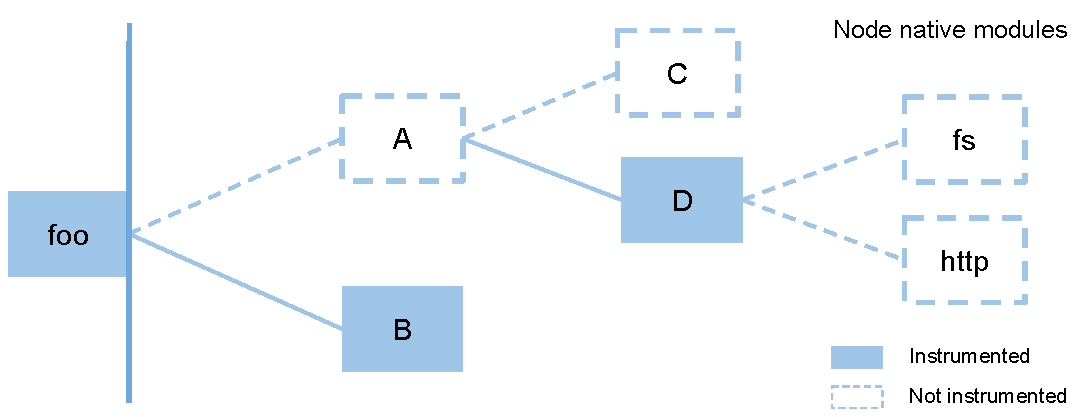
\includegraphics[width=1\textwidth]{figures/approach/blacklisted-modules/blacklisted-modules.pdf}}
	
	\caption[Non-instrumented node modules]{\textbf{Non-instrumented node modules} - Dependencies tree for module \textit{foo}. Modules \textit{A} and \textit{B} are included in the blacklist. Module \textit{D} is instrumented anyway, even though its parent is not. Node native modules, like \textit{fs} or \textit{http}, are excluded anyway by Jalangi.}
	\label{fig:blacklisted-modules}
\end{figure}
\todo{Incluir grafico con los blacklisted modules}

\subsection{Implementation}
\todo{NodeJS \& Docker. Mostrar cómo se invoca, etc.}

\section{TypeScript Declaration File Generation}
\todo{Tres tipos de modulos en TypeScript}
\todo{Traceids y que las signatures de las funciones no se unen, sino que se acumulan segun traceId. Obviamente las iguales no se escriben de vuelta.}
\todo{El nombre de las interfaces se crea con el nombre de la variable}
\todo{El tipo se extrae del valor en runtime.}
\subsection{Implementation}
\todo{TypeScript \& Docker. Mostrar cómo se invoca, etc.}

\section{Evaluation}
\begin{figure}[h]
\begin{centering}
    {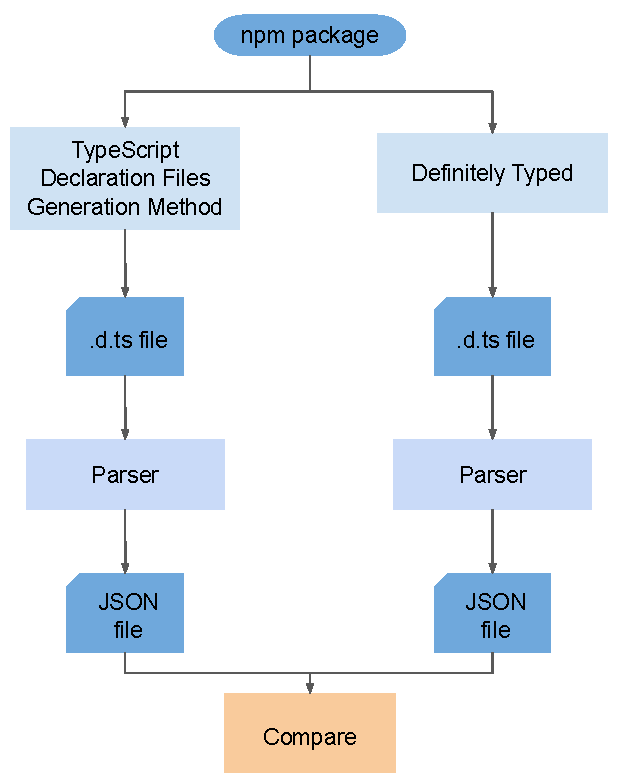
\includegraphics[width=0.8\textwidth]{figures/approach/evaluation/evaluation-diagram.pdf}}
    \caption[Evaluation against DefinitelyTyped Repository]{\textbf{Evaluation of generated declaration files against DefinitelyTyped Repository} - A parser transforms the generated declaration file and the equivalent file in the DefinitelyTyped repository into a JSON file using the TypeScript Compiler API \citep{typescript-compiler-api}. Comparison is then performed on the JSON files, i.e. not on the declaration files.}
    \label{fig:evaluation-diagram}
\end{centering}
\end{figure}

\subsection{Parsing}
\subsubsection{TypeScript Compiler API}
\subsection{Comparison}
\todo{Number of functions}
\todo{Number of parameters}
\todo{Interfaces}
\todo{methodCall}
\todo{usedAsArgument}
\todo{Syntax \& Semantic Errors}